%Xiaowen Chang, April 2016

\documentclass[10pt,letter]{article}
	% basic article document class
	% use percent signs to make comments to yourself -- they will not show up.

\usepackage{amsmath}
\usepackage{amssymb}
	% packages that allow mathematical formatting

\usepackage{graphicx}
	% package that allows you to include graphics

\usepackage{setspace}
	% package that allows you to change spacing

\onehalfspacing
	% text become 1.5 spaced

\usepackage{fullpage}
	% package that specifies normal margins

\usepackage{hyperref}

\usepackage{subfig}

\usepackage{verbatim}

\usepackage[parfill]{parskip}

\usepackage{listings}

\usepackage{color}

\usepackage{booktabs}

\usepackage{multirow}

\usepackage{longtable}

\usepackage{common}

\usepackage{fancyhdr}
\pagestyle{fancy}
\voffset = -2em
\headsep = 25pt %1.5em
\lhead{\textsc{Team Name: Black Jack}}
\rhead{\textsc{Now I See You}}

\numberwithin{equation}{section} % Number equations within sections (i.e. 1.1, 1.2, 2.1, 2.2 instead of 1, 2, 3, 4)
\numberwithin{figure}{section} % Number figures within sections (i.e. 1.1, 1.2, 2.1, 2.2 instead of 1, 2, 3, 4)
\numberwithin{table}{section} % Number tables within sections (i.e. 1.1, 1.2, 2.1, 2.2 instead of 1, 2, 3, 4)
 
\hypersetup{hidelinks=true}

\allowdisplaybreaks

\begin{document}

\begin{titlepage}

\newcommand{\HRule}{\rule{\linewidth}{0.5mm}} % Defines a new command for the horizontal lines, change thickness here
%----------------------------------------------------------------------------------------
%	LOGO SECTION
%----------------------------------------------------------------------------------------


\includegraphics[width=7cm]{logo.png}\\[2cm] 
\center % Center everything on the page
%----------------------------------------------------------------------------------------
%	HEADING SECTIONS
%----------------------------------------------------------------------------------------

\textsc{\Huge AM 207 Final Project}\\[1.5cm] % Name of your university/college
\textsc{\LARGE Now I See You}\\[0.5cm] % Major heading such as course name
\textsc{\Large Sensor Based Singer User Activity Recognition}\\[3cm] % Minor heading such as course title
 
%----------------------------------------------------------------------------------------
%	AUTHOR SECTION
%----------------------------------------------------------------------------------------

\begin{minipage}{0.4\textwidth}
\center \large
\emph{Group Members:}\\[0.4cm]
Xiaowen \textsc{Chang} \\
Baijie \textsc{Lu}\\ 
Fangzheng \textsc{Qian} \\
Yuhan \textsc{Tang} 
% Your name
\end{minipage}
 
%----------------------------------------------------------------------------------------

\vfill % Fill the rest of the page with whitespace

\end{titlepage}

\section{Introduction}
Activity Recognition, which identifies the activity (eg. cooking, sleeping, reading) that a user performs from a series of observations, is an active research area because it has many real-life applications such as healthcare and intelligent environments. In our project, to simplify the problem, we used sensor based singer user data instead of some complex activities data involved multiple users. Recognize activities from sensor data poses the following challenges. First, there is an ambiguity of interpretation. The interpretation of similar observed sensor data may be different. For example, 'cooking' and 'cleaning fridge' both involve opening the fridge. Second, same activity may be performed in different ways. Third, from the observed sensor data, it is hard to see when one activity ends and another one starts. In this project, we implemented Naive Bayes Model, First Order HMM(Hidden Markov Model) and Second Order HMM to tackle these issues and tested their performance on several real world datasets. Besides models, different feature representations were tried to further improve the performance. 

\section{Data}
In this project, supervised machine learning models were used for recognition of users' activity, therefore, labeled training data from sensors had to be collected. We used three online datasets with single user activity recorded in different houses. Sensors were installed in different places inside the house to gather the data needed for recognition. The floor plan of different houses is as following. The red boxes represent sensor nodes. It gives 1 when the sensor is firing and a 0 otherwise. 
\begin{figure}[h]
    \centering
    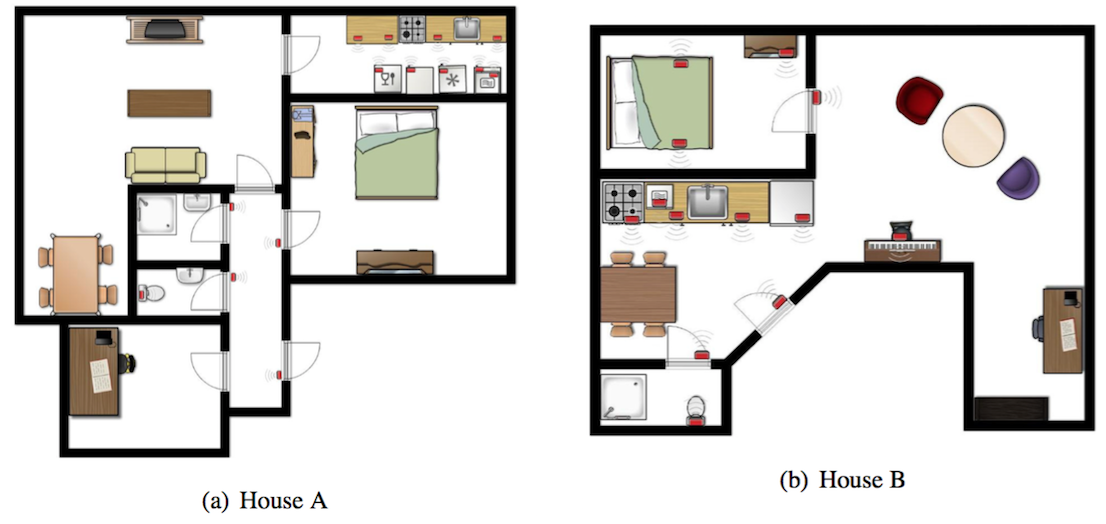
\includegraphics[width=16cm]{data1}
\end{figure}
\newpage
\begin{figure}[h]
    \centering
    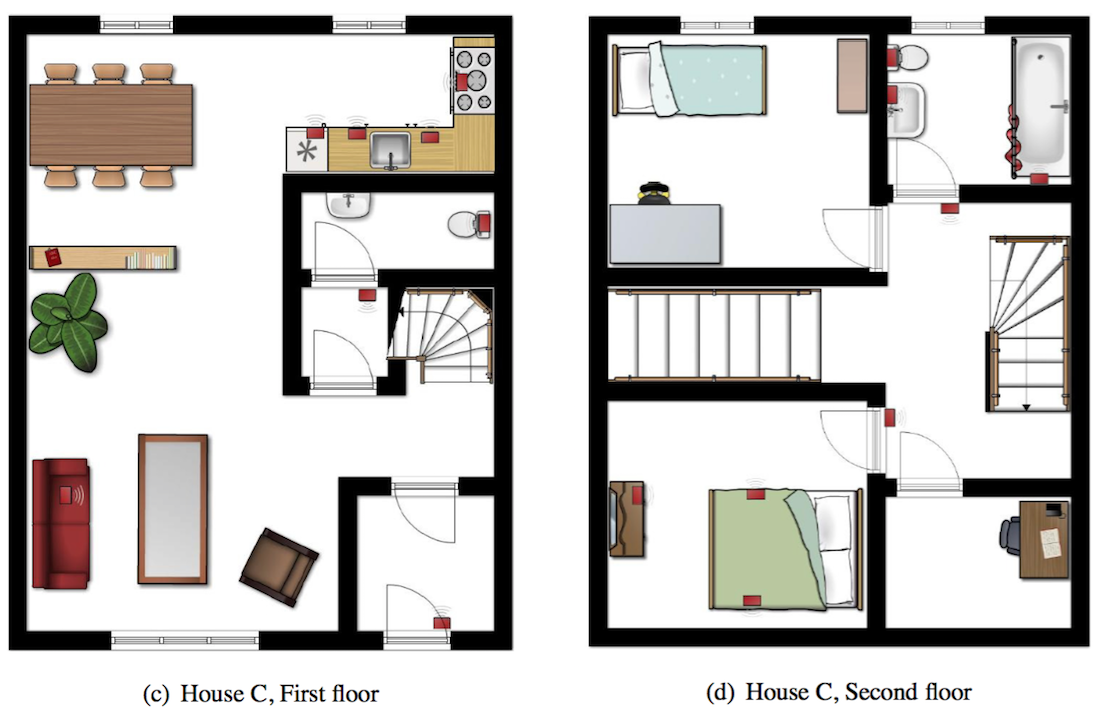
\includegraphics[width=14cm]{data2}
\end{figure}
To test our model performance, we left one day out as test data and the remaining days were used for training. To avoid overfitting, we used cross validation approach to cycle over all the days and report the average performance. 

After some experiments, data was discretized into T time slices of length $\Delta t =60$ seconds which is long enough to be discriminative and gives a relative small discretization error. When two or more activities occur within a single time slice, we used the activity that occupies most of the time slice.  In a house dataset, with N sensors installed, we define a binary observation state vector at time t as $x_{t} = (x_{t1}, x_{t2}, ... , x_{tN})^T$. The hidden state(activity) is denoted with $y_t \in \{1,2, ..., D\}$ for D possible hidden states. We want to map from $x_t$ to $y_t$ so that through observed sensor data at time t we could recognize the user's activity.
\section{Model and Algorithm}
\subsection{Assumption and Parameter Estimation}
The exact distribution of the observation would require $2^N$ parameters with N being the number of sensors used.  To simplify the problem, we applied Naive Bayes conditional independence assumption to all of our models, which means given the hidden state(activity) label the features are independent, i.e. 
$$P(x_t|y_t = i) = \prod_{n=1}^N P(x_{tn}|y_t=i)$$ which requires only N parameters for each activity.

Also, we modeled each sensor observation as an independent Bernoulli distribution so that 
$$P(x_{tn}|y_t = i) = \mu_{ni}^{x_{tn}}(1-\mu_{ni})^{1-x_{tn}}$$
The parameter $\mu_{ni}$ of each model could be learned  by maximizing likelihood(MLE), that is we find the $\hat{\mu}_{ni}$ that could maximize 
$$\prod_{t=1}^T P(x_{tn}|y_t = i) = \prod_{t=1}^T \mu_{ni}^{x_{tn}}(1-\mu_{ni})^{1-x_{tn}}$$
Then the estimation is given by:
$$\hat{\mu}_{ni} = \frac{\sum_{t=1}^T x_{tn}\mathbf{1}\{y_t=i\}}{\sum_{t=1}^T \mathbf{1}\{y_t=i\}}$$
The MLE estimator considers the parameter to be a constant and estimates a value that provide maximum support for the data.

\subsection{Naive Bayes Model}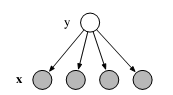
\includegraphics[width=7cm]{NB}
Besides the conditional independence assumption, Naive Bayes Model also assumes all data points are independently and identically distributed, that is it doesn't consider the correlation between data points. 
The joint probability over the testing data points:
$$P(X_{1:T}|Y_{1:T})= \prod_{t=1}^T P(x_t|y_t)P(y_t)= \prod_{t=1}^T\prod_{n=1}^N\prod_{i=1}^D P(x_{tn}|y_t = i)P(y_t=i)$$
$$ = \prod_{t=1}^T\prod_{n=1}^N\prod_{i=1}^D  \pi_{ti}*\mu_{ni}^{x_{tn}}(1-\mu_{ni})^{1-x_{tn}}$$
where $\pi_{ti}$ is based on the frequencies of activity i during time slot t in the training data without taking any observed sensor data into account. \\
MLE estimates for $\pi_{ti}$ are
$$\hat{\pi}_{ti} = \frac{|S\{y_t=i\}|} {|S|}$$
where $|S|$ denotes the number of elements in the training set S.\\
By maximizing the product of the joint probability with respect to $y_{1:T} = \{y_1,y_2,...,y_T\}$ over the data points, we could find a mapping between the observation data $x_{1:T} = \{x_1,x_2,...x_T\}$ and a sequence of activity labels $y_{1:T} = \{y_1,y_2,...,y_T\}$.
\newpage
To give you a sense of how the prior distribution looks like, we plot the prior probability $P(y= sleeping)$ over different time slots as below: \\
\begin{figure}[h]
    \centering
    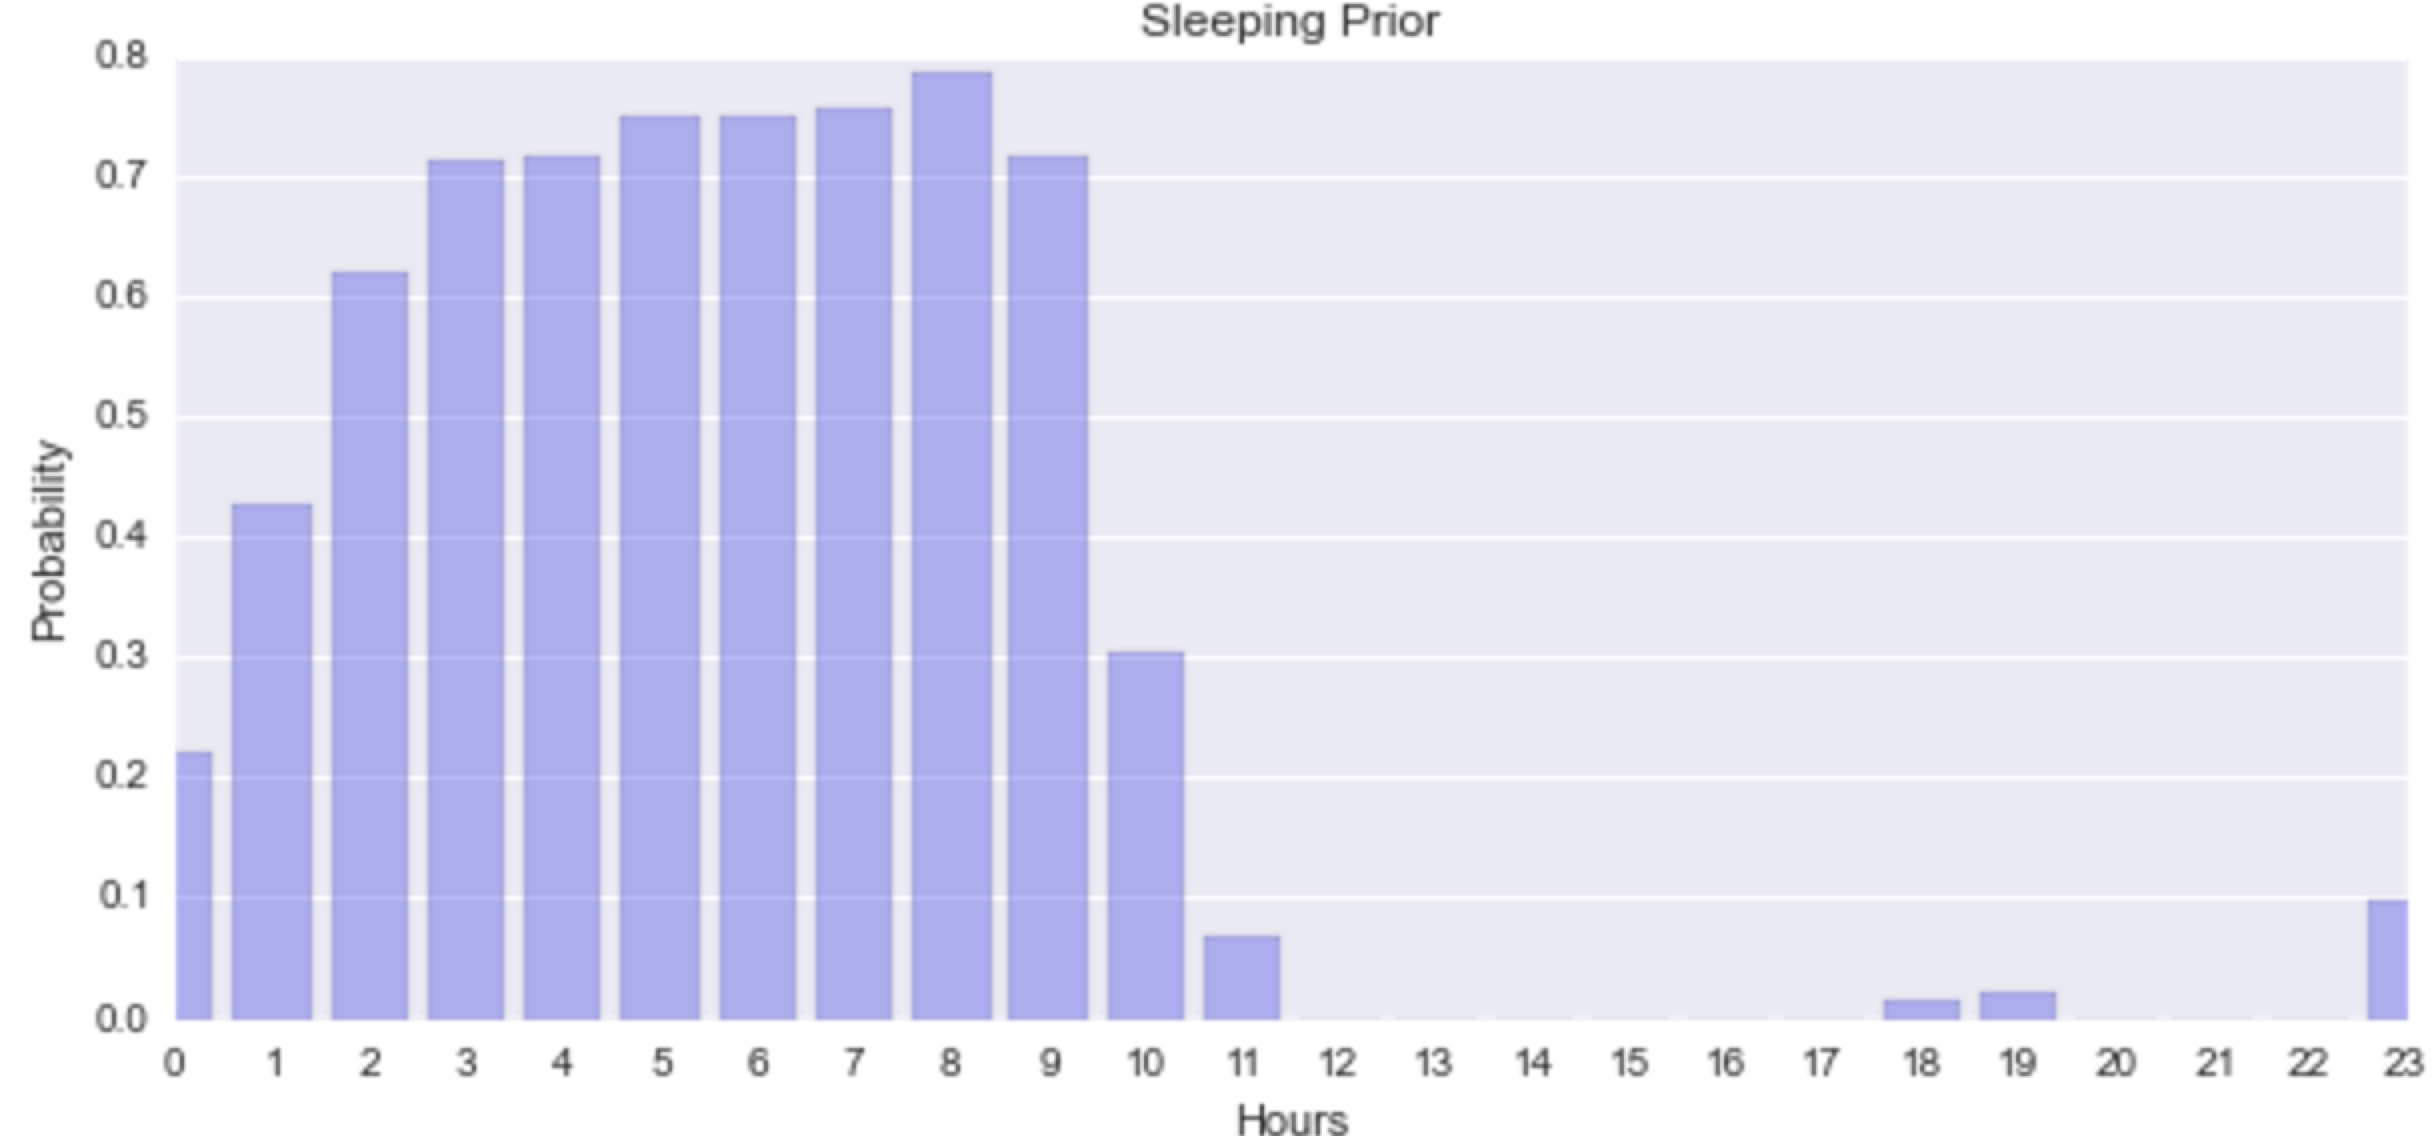
\includegraphics[width=18cm]{sleeping_prior}
\end{figure}\\
To visualize the performance of this Naive Bayes model, we plotted the prior probability, posterior probability and true probability of the activity 'go to bed' during different hours using our testing data. This plot could show us how did Naive Bayes model improved the prediction by taking observed sensor data into account.
\begin{figure}[h]
    \centering
    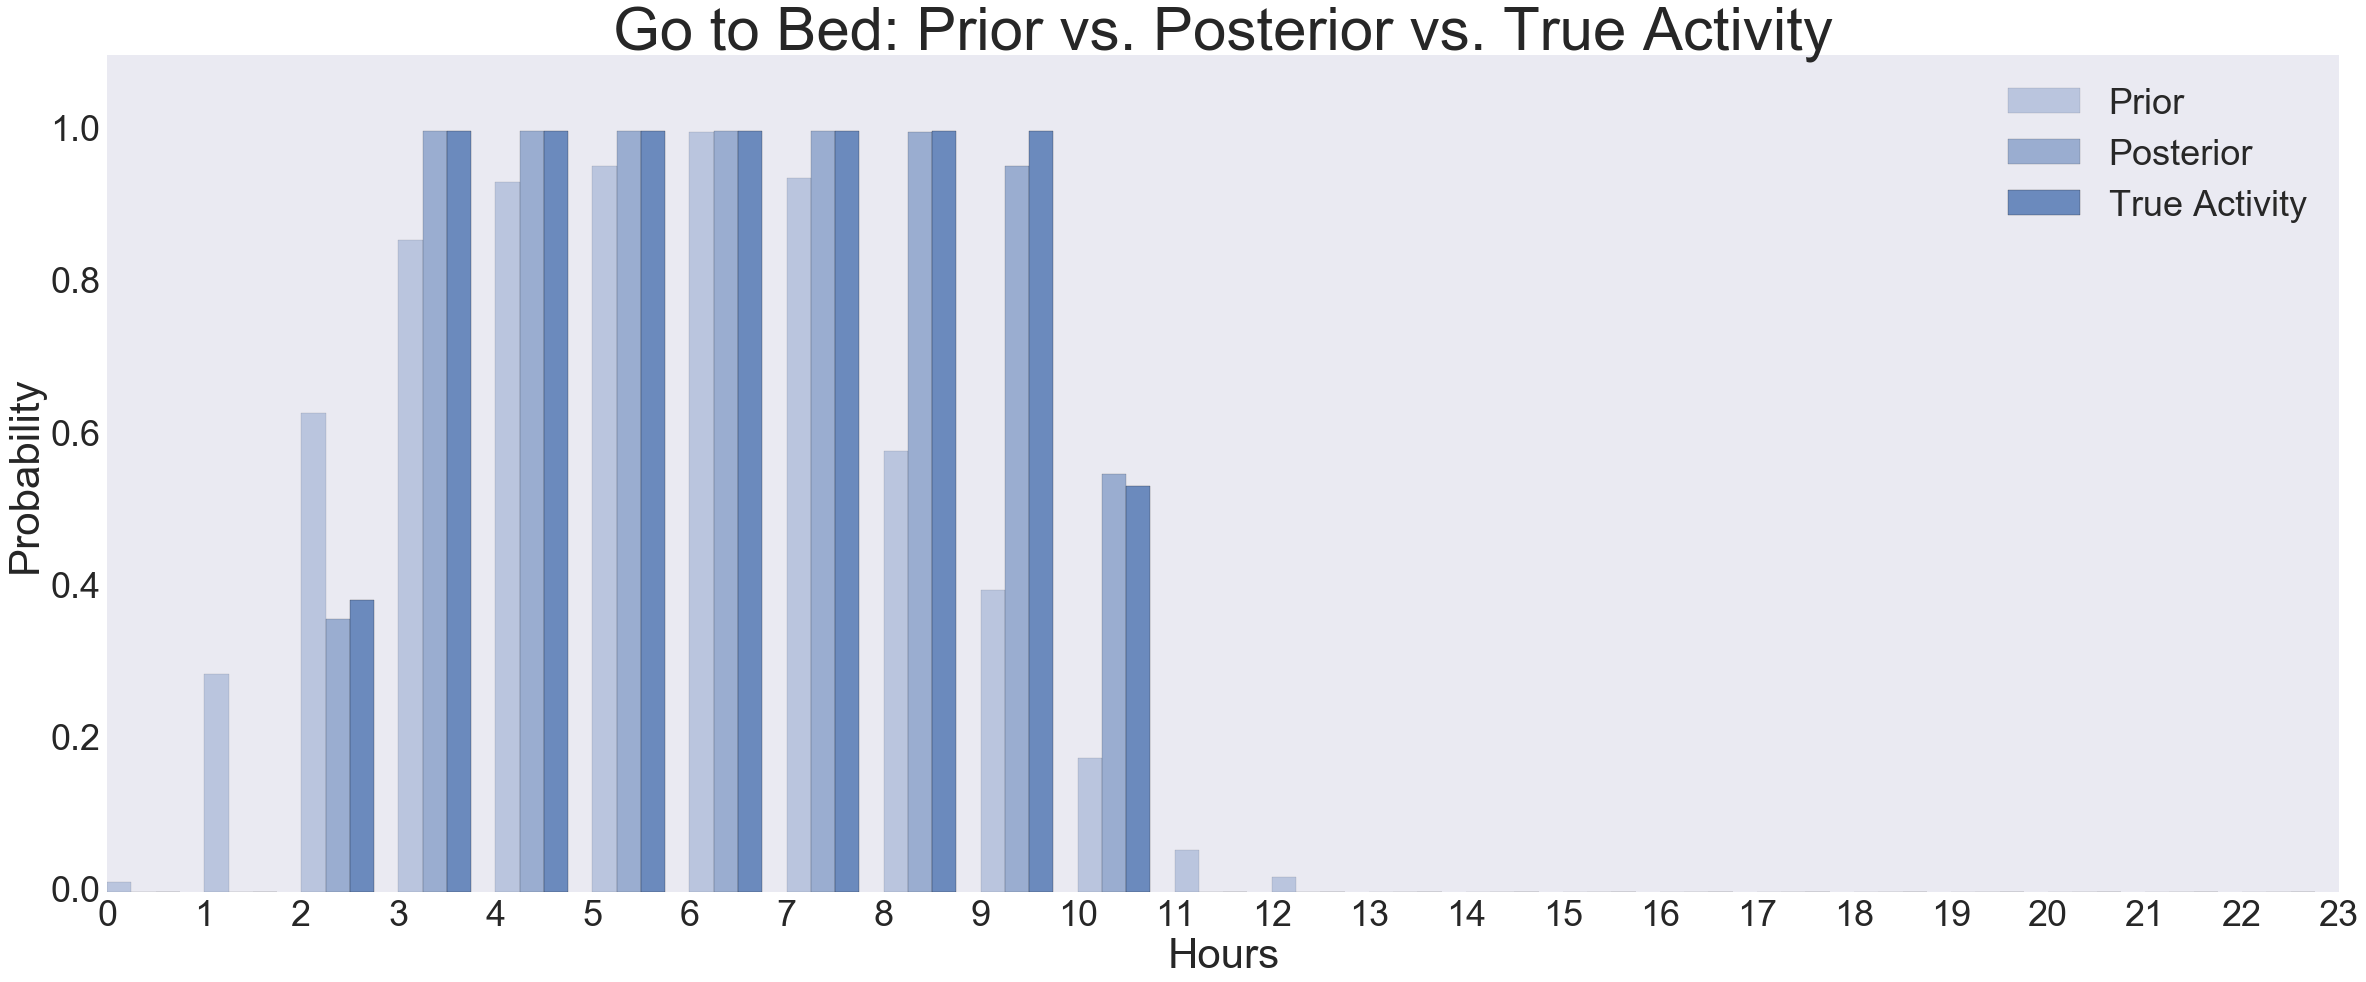
\includegraphics[width=18cm]{NB_result}
\end{figure}
\subsection{First Order HMM (Hidden Markov Model)}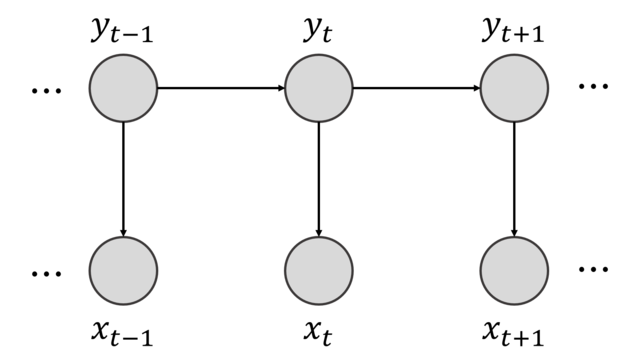
\includegraphics[width=7cm]{1hmm}
In Naive Bayes model, we assumes all data points are independently and identically distributed. However, it is not true. The data we have are time series data and there exists a temporal correlation between consecutive time slices. A Hidden Markov Model (HMM) can be used to explore this scenario. In an HMM model, we have a series of observed outputs $X={x_1, x_2, ...,x_t}$ drawn from a series of hidden state $Y={y_1, y_2, ..,y_t}$. In this problem, X should be the observed sensor states and Y should be the activity states. The First Order HMM relies on the following three assumptions:
\begin{itemize}
\item \textbf{Limited Horizon Assumption:} the probability of being in a hidden state at time t depends only on the hidden state at time t-1.
\item \textbf{Stationary Process Assumption:} the conditional distribution over next hidden state given current hidden state does not change over time. P
\item \textbf{Output Independence Assumption:} the output observation at time t is dependent
only on the current hidden state.
\end{itemize}
From this HMM, we want to know what is the most likely series of states  $y_{1:T} = \{y_1,y_2,...,y_T\}$ given an observed series of observed sensor data $x_{1:T} = \{x_1,x_2,...x_T\}$. Formally, we seek:
$$arg max_{Y} P(Y|X; A, B) = arg max_{Y} \prod_{t=1}^{T} \frac{P(y_t, x_t; A, B)}{\sum_{Y} P(y_t,x_t; A,B)}= arg max_{Y} \prod_{t=1}^{T} P(y_t, x_t; A, B)$$
$$ \prod_{t=1}^{T} P(y_t, x_t) = \prod_{t=1}^T P(x_t|y_t)P(y_t|y_{t-1})=\prod_{t=1}^T\prod_{n=1}^N\prod_{i=1}^D P(x_{tn}|y_t = i)P(y_t=i|y_{t-1})$$
where A is the transition matrix and B is the emission matrix. To simplify the notation, we used $P(y_1|y_0)=P(y_1)$. The element $a_{ij}$ in matrix A represents $P(y_t=j|y_{t-1}=i)$. The element $b_{in}$ in matrix B represents $P(x_{tn}|y_t=i)$, which is equivalent to $\mu_{ni}$.  The transition probability $a_{ij}=P(y_t=j|y_{t-1}=i)$ is a multinomial distribution and $a_{ij}$ is given by:
$$\hat{a}_{ij} = \frac{\sum_{t=1}^T \mathbf{1}\{y_t=j\}\mathbf{1}\{y_{t-1}=i\}}{\sum_{t=1}^T \mathbf{1}\{y_{t-1}=i\}}$$
To solve the argmax equation, naively, we could try every possible assignment to Y and take the one with highest value of joint probability. However, it would require $\mathcal{O}(|Y|^T)$ operations. So instead, we used a dynamic programming algorithm called Viterbi to solve this equation. 

\subsection{Second Order HMM (Hidden Markov Model)}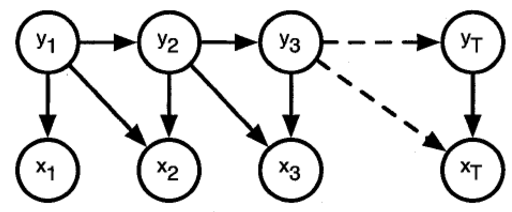
\includegraphics[width=7cm]{2hmm}
The order of a HMM is the length of history upon which the probabilities of the possible values of the next state depend. The only difference between 1st and 2nd order HMM is that 2nd order HMM depends upon the two previous states. Thus, the probability of transitioning to a new state depends not only on the current state, but also on the previous state. This allows a more realistic context dependence.

We could rewrite our likelihood as following:
$$ \prod_{t=1}^{T} P(y_t, x_t) = \prod_{t=1}^T P(x_t|\{y_t, y_{t-1}\})P(\{y_t,y_{t-1}\}|\{y_{t-1},y_{t-2}\})$$
$$=\prod_{t=1}^T\prod_{n=1}^N\prod_{\{i,j\}=\{1,1\}}^{D^2} P(x_{tn}|\{y_t, y_{t-1}\} = \{i,j\})P(\{y_t, y_{t-1}\} = \{i,j\}|\{y_{t-1}, y_{t-2}\}) $$
We could used the same Viterbi algorithm as 1st order HMM with different Transition matrix and Emission matrix to find the maximum likelihood assignment for 2nd order HMM. 
Instead of using D different activities as our hidden states, we used all combinations of 2 activities as our hidden states in 2nd order HMM, which has a size of $D^2$. Thus,
$$\hat{a}_{ij, jk} = \frac{\sum_{t=2}^T \mathbf{1}\{\{y_t,y_{t-1}\}=\{j,k\}\}\mathbf{1}\{\{y_{t-1},y_{t-2}\}=\{i,j\}\}}{\sum_{t=2}^T \mathbf{1}\{\{y_{t-1},y_{t-2}\}=\{i,j\}\}}$$
$$\hat{b}_{ij,n} = \frac{\sum_{t=1}^T x_{tn}\mathbf{1}\{\{y_t,y_{t-1}\}=\{i, j\}\}}{\sum_{t=1}^T \mathbf{1}\{\{y_t,y_{t-1}\}=\{i, j\}\}}$$

\section{Feature Representation}
\begin{figure}[h]
\centering
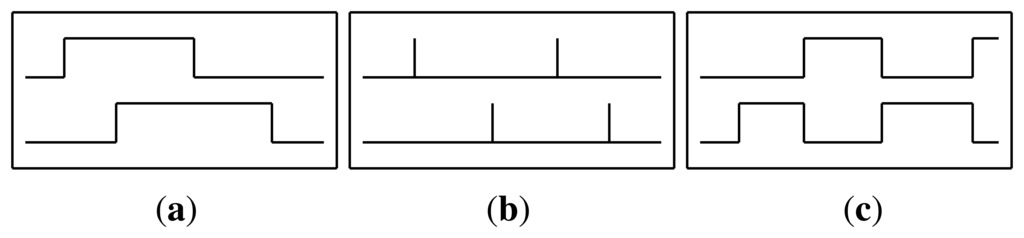
\includegraphics[width=14cm]{feature}
\caption{ (a) Raw; (b) ChangePoint; (c) LastSensor}
\end{figure}
Besides models, we also tried different feature representation to improve our prediction performance. 
As shown in the graph above, 
\\(a) is our raw data feature representation which gives 1 when the sensor is firing and a 0 otherwise.  
\\(b) is ChangePoint feature representation, which indicates the moment when a sensor changes its value. 
\\(c) is LastSensor feature representation. It indicates which sensor fired last. The sensor that changed state last continues to give 1 and only changes to 0 when another sensor changes its value.

\section{Model Comparison}
To evaluate the performance of different models with different feature representations, we used the following four metrics:
\begin{itemize}
\item \textbf{Precision:} the number of True Positives divided by the number of True Positives and False Positives.
$$\text{Precision} = \frac{1}{N}\sum^N_i \frac{TP_i}{TP_i+FP_i} $$
\item \textbf{Recall:} the number of True Positives divided by the number of True Positives and the number of False Negatives.
$$\text{Recall} = \frac{1}{N}\sum^N_i\frac{TP_i}{TP_i + FN_i} $$
\item \textbf{F-Measure:} conveys the balance between the precision and the recall.
$$\text{F-Measure} = \frac{2 \cdot precision \cdot recal}{precision+recall} $$
\item \textbf{Accuracy:} the number of True Positives and True Negatives divided by the total number.
$$\text{Accuracy} = \frac{\sum^N_i TP_i + TN_i}{Total}$$
\end{itemize}
Using the four metrics above to visualize the performance of our models, we plotted the performance heat map for different houses. Here we used the performance heat map of house C as an example:\\
\textbf{heat map plot here}
\\
Naive Bayes is the simplest model without taking time factor into account while HMM add temporal relations. However, from the result above, we did not see a significant performance improvement. This might be because HMM model needs more training data to accurately learn the parameters. 

Also we noticed that the choice of feature representation strongly affects the recognition performance. It is hard to see when one activity ends and another one starts using raw data feature representation and it does not provide good information about the activity currently performed. For example, the observed open his laptop doing some work and then go to sleep without closing his laptop then the raw representation can indicate that the laptop is open long after the person finished using the laptop. The ChangePoint representation can solve this issue because it only indicates the moment the sensor changes its value, however, unless another sensor fired, it can not differentiate whether the person is currently doing the activity or already finished. LastSensor representation solved this issue and thus gives us the best results.  

In terms of future work, more complex model like Hidden semi-Markov model, Conditional Random Fields, Neutral Network could be tried to improve the recognition performance. 

\end{document}
	% line of code telling latex that your document is ending. If you leave this out, you'll get an error